%%%
%%%
\documentclass[12pt]{extarticle}
\usepackage{fullpage,latexsym,picinpar,amsmath,amsfonts, amsthm, pgfplots}
\usetikzlibrary{patterns}
           

%%%%%%%%%%%%%%%%%%%%%%%%%%%%%%%%%%%%%%%%%%%%%%%%%%%%%%%%%%%%%%%%%%%%%%%%%%%%%%%%%%%
%%%%%%%%%%%  LETTERS 
%%%%%%%%%%%%%%%%%%%%%%%%%%%%%%%%%%%%%%%%%%%%%%%%%%%%%%%%%%%%%%%%%%%%%%%%%%%%%%%%%%%

\newcommand{\barx}{{\bar x}}
\newcommand{\bary}{{\bar y}}
\newcommand{\barz}{{\bar z}}
\newcommand{\bart}{{\bar t}}

\newcommand{\bfP}{{\bf{P}}}

%%%%%%%%%%%%%%%%%%%%%%%%%%%%%%%%%%%%%%%%%%%%%%%%%%%%%%%%%%%%%%%%%%%%%%%%%%%%%%%%%%%
%%%%%%%%%%%%%%%%%%%%%%%%%%%%%%%%%%%%%%%%%%%%%%%%%%%%%%%%%%%%%%%%%%%%%%%%%%%%%%%%%%%
                                                                                
\newcommand{\parend}[1]{{\left( #1  \right) }}
\newcommand{\spparend}[1]{{\left(\, #1  \,\right) }}
\newcommand{\angled}[1]{{\left\langle #1  \right\rangle }}
\newcommand{\brackd}[1]{{\left[ #1  \right] }}
\newcommand{\spbrackd}[1]{{\left[\, #1  \,\right] }}
\newcommand{\braced}[1]{{\left\{ #1  \right\} }}
\newcommand{\leftbraced}[1]{{\left\{ #1  \right. }}
\newcommand{\floor}[1]{{\left\lfloor #1\right\rfloor}}
\newcommand{\ceiling}[1]{{\left\lceil #1\right\rceil}}
\newcommand{\barred}[1]{{\left|#1\right|}}
\newcommand{\doublebarred}[1]{{\left|\left|#1\right|\right|}}
\newcommand{\spaced}[1]{{\, #1\, }}
\newcommand{\suchthat}{{\spaced{|}}}
\newcommand{\numof}{{\sharp}}
\newcommand{\assign}{{\,\leftarrow\,}}
\newcommand{\myaccept}{{\mbox{\tiny accept}}}
\newcommand{\myreject}{{\mbox{\tiny reject}}}
\newcommand{\blanksymbol}{{\sqcup}}
                                                                                                                         
\newcommand{\veps}{{\varepsilon}}
\newcommand{\Sigmastar}{{\Sigma^\ast}}
                           
\newcommand{\half}{\mbox{$\frac{1}{2}$}}    
\newcommand{\threehalfs}{\mbox{$\frac{3}{2}$}}   
\newcommand{\domino}[2]{\left[\frac{#1}{#2}\right]}  

%%%%%%%%%%%% complexity classes

\newcommand{\PP}{\mathbb{P}}
\newcommand{\NP}{\mathbb{NP}}
\newcommand{\PSPACE}{\mathbb{PSPACE}}
\newcommand{\coNP}{\textrm{co}\mathbb{NP}}
\newcommand{\DLOG}{\mathbb{L}}
\newcommand{\NLOG}{\mathbb{NL}}
\newcommand{\NL}{\mathbb{NL}}

%%%%%%%%%%% decision problems

\newcommand{\PCP}{\sc{PCP}}
\newcommand{\Path}{\sc{Path}}
\newcommand{\GenGeo}{\sc{Generalized Geography}}

\newcommand{\malytm}{{\mbox{\tiny TM}}}
\newcommand{\malycfg}{{\mbox{\tiny CFG}}}
\newcommand{\Atm}{\mbox{\rm A}_\malytm}
\newcommand{\complAtm}{{\overline{\mbox{\rm A}}}_\malytm}
\newcommand{\AllCFG}{{\mbox{\sc All}}_\malycfg}
\newcommand{\complAllCFG}{{\overline{\mbox{\sc All}}}_\malycfg}
\newcommand{\complL}{{\bar L}}
\newcommand{\TQBF}{\mbox{\sc TQBF}}
\newcommand{\SAT}{\mbox{\sc SAT}}

%%%%%%%%%%%%%%%%%%%%%%%%%%%%%%%%%%%%%%%%%%%%%%%%%%%%%%%%%%%%%%%%%%%%%%%%%%%%%%%%%%%
%%%%%%%%%%%%%%% for homeworks
%%%%%%%%%%%%%%%%%%%%%%%%%%%%%%%%%%%%%%%%%%%%%%%%%%%%%%%%%%%%%%%%%%%%%%%%%%%%%%%%%%%

\newcommand{\student}[2]{%
{\noindent\Large{ \emph{#1} SID {#2} } \hfill} \vskip 0.1in}

\newcommand{\assignment}[1]{\medskip\centerline{\large\bf CS 111 ASSIGNMENT {#1}}}

\newcommand{\duedate}[1]{{\centerline{due {#1}\medskip}}}     

\newcounter{problemnumber}                                                                                 

\newenvironment{problem}{{\vskip 0.1in \noindent
              \bf Problem~\addtocounter{problemnumber}{1}\arabic{problemnumber}:}}{}

\newcounter{solutionnumber}

\newenvironment{solution}{{\vskip 0.1in \noindent
             \bf Solution~\addtocounter{solutionnumber}{1}\arabic{solutionnumber}:}}
				{\ \newline\smallskip\lineacross\smallskip}

\newcommand{\lineacross}{\noindent\mbox{}\hrulefill\mbox{}}

\newcommand{\decproblem}[3]{%
\medskip
\noindent
\begin{list}{\hfill}{\setlength{\labelsep}{0in}
                       \setlength{\topsep}{0in}
                       \setlength{\partopsep}{0in}
                       \setlength{\leftmargin}{0in}
                       \setlength{\listparindent}{0in}
                       \setlength{\labelwidth}{0.5in}
                       \setlength{\itemindent}{0in}
                       \setlength{\itemsep}{0in}
                     }
\item{{{\sc{#1}}:}}
                \begin{list}{\hfill}{\setlength{\labelsep}{0.1in}
                       \setlength{\topsep}{0in}
                       \setlength{\partopsep}{0in}
                       \setlength{\leftmargin}{0.5in}
                       \setlength{\labelwidth}{0.5in}
                       \setlength{\listparindent}{0in}
                       \setlength{\itemindent}{0in}
                       \setlength{\itemsep}{0in}
                       }
                \item{{\em Instance:\ }}{#2}
                \item{{\em Query:\ }}{#3}
                \end{list}
\end{list}
\medskip
}

%%%%%%%%%%%%%%%%%%%%%%%%%%%%%%%%%%%%%%%%%%%%%%%%%%%%%%%%%%%%%%%%%%%%%%%%%%%%%%%%%%%
%%%%%%%%%%%%% for quizzes
%%%%%%%%%%%%%%%%%%%%%%%%%%%%%%%%%%%%%%%%%%%%%%%%%%%%%%%%%%%%%%%%%%%%%%%%%%%%%%%%%%%

\newcommand{\quizheader}{ {\large NAME: \hskip 3in SID:\hfill}
                                \newline\lineacross \medskip }


%%%%%%%%%%%%%%%%%%%%%%%%%%%%%%%%%%%%%%%%%%%%%%%%%%%%%%%%%%%%%%%%%%%%%%%%%%%%%%%%%%%
%%%%%%%%%%%%% for final
%%%%%%%%%%%%%%%%%%%%%%%%%%%%%%%%%%%%%%%%%%%%%%%%%%%%%%%%%%%%%%%%%%%%%%%%%%%%%%%%%%%

\newcommand{\namespace}{\noindent{\Large NAME: \hfill SID:\hskip 1.5in\ }\\\medskip\noindent\mbox{}\hrulefill\mbox{}}



%\pagestyle{empty}

\usepackage[hidelinks]{hyperref} 
\usepackage{makeidx}
\usepackage{enumerate}
\usepackage{stmaryrd}
\usepackage{mathrsfs}
\usepackage{mdframed}
\usepackage{lipsum}
\usepackage{anyfontsize}
\everymath{\displaystyle}
%
\textwidth 6in
\oddsidemargin 0.25in
\evensidemargin 0.25in 
%
\title{Math 120 Optimization: Homework 3}
\author{Stanley Cohen}
%\address{Department of Mathematics, Vanderbilt University, 1326 Stevenson Center, Nashville, TN 37240}
%\email{chenxu.wen@vanderbilt.edu}
\date{}
%\thanks{}
%\subjclass{}
%\renewcommand{\subjclassname}{\textup{2000} Mathematics Subject Classification}
%\keywords{}
%\dedicatory{}

%\makeindex

%
\newtheorem{thm}{Theorem}
\newtheorem*{thm*}{Theorem}
\newtheorem*{cor*}{Corollary}
\newtheorem{prop}[thm]{Proposition}
\newtheorem{cor}[thm]{Corollary}
\newtheorem{lem}[thm]{Lemma}
\theoremstyle{definition}
\newtheorem{defn}[thm]{Definition}
\newtheorem{rem}[thm]{Remark}
\newtheorem{examp}[thm]{Example}
\newtheorem{claim}[thm]{Claim}
\newtheorem{exer}[thm]{Exercise}
\newtheorem{prob}[thm]{Problem}
\newtheorem{open}[thm]{Open Problem}
\newtheorem{note}[thm]{Notation}
\newtheorem{que}[thm]{Question}
\def\R{{\mathbb{R}}}


%
\newcommand{\actson}{{\curvearrowright}}
\newcommand{\pgfplotsdrawaxis}{\pgfplots@draw@axis}
\makeatother
\pgfplotsset{only axis on top/.style={axis on top=false, after end axis/.code={
             \pgfplotsset{axis line style=opaque, ticklabel style=opaque, tick style=opaque,
                          grid=none}\pgfplotsdrawaxis}}}

\newcommand{\drawge}{-- (rel axis cs:1,0) -- (rel axis cs:1,1) -- (rel axis cs:0,1) \closedcycle}
\newcommand{\drawle}{-- (rel axis cs:1,1) -- (rel axis cs:1,0) -- (rel axis cs:0,0) \closedcycle}




%
\begin{document}



\maketitle

\begin{problem}
 Convert the following linear programming problem into \textit{standard form}:
\begin{align*}
\text{maximize } &2x_1+x_2\\
\text{subject to } &0\leq x_1\leq 2\\
&x_1+x_2\leq 3\\
&x_1+2x_2\leq 5\\
&x_2\geq 0.
\end{align*}

We can add some variables to turn the inequalities into equalities so the problem becomes:

\begin{align*}
\text{maximize } &2x_1+x_2\\
\text{subject to } &x_1 + s_1 = 2\\
&x_1 + x_2 + s_2 = 3\\
&x_1 + 2x_2 + s_3 = 5\\
&x_1, x_2, s_1, s_2, s_3 \geq 0.
\end{align*}

\end{problem}


\begin{problem}
 Suppose that a computer supplier has two warehouses, one located in city A and another in city B. The supplier receives orders from two customers, one in city C and another in city D. The customer in city C orders 50 units, and the customer in city D orders 60 units. The number of units at the warehouse in city A is 70 and the number of units at the warehouse in city B is 80. The cost of shipping each unit from A to C is 1, from A to D is 2, from B to C is 3, from B to D is 4.



 	\begin{description}
		\item{(a)} Formulate the problem of deciding how many units from each warehouse should 
		be shipped to each customer to minimize the total shipping cost.

			\textit{(Not sure what ``Formulate the problem'' means, but hopefully this will work?)}

			Let $x_y$ be the number of items shipped from warehouse $x$ to city $y$.

			\begin{align*}
			\text{minimize } &a_c + 2a_d + 3b_c + 4b_d\\
			\text{subject to } &a_c + a_d \leq 70\\
			&b_c + b_d \leq 80\\
			&a_c + b_c = 50\\
			&a_d + b_d = 60.
			\end{align*} 

		\item{(b)} Express the problem as an equivalent standard form linear programming problem.

			We can add some variables to turn the inequalities into equalities so the problem becomes:
			
			\begin{align*}
			\text{minimize } &a_c + 2a_d + 3b_c + 4b_d\\
			\text{subject to } &a_c + a_d + s_1 = 70\\
			&b_c + b_d + s_2 = 80\\
			&a_c + b_c = 50\\
			&a_d + b_d = 60\\
			&a_c, a_d, b_c, b_d, s_1, s_2 \geq 0.
			\end{align*} 


	\end{description}
\end{problem}


\begin{problem}
	 A cereal manufacturer wishes to produce 1000 pounds of a cereal that contains exactly 10\% fiber, 2\% fat, and 5\% sugar (by weight). The cereal is to be produced by combining four items of raw food material in appropriate proportions. These four items are named $a, b, c, d$ and they have certain combinations of fiber, fat, and sugar content, and are available at various prices per pound:
	\begin{center}
	 \begin{tabular}{||c | c c c c||} 
	 \hline
	 Item  & $a$ & $b$ & $c$ & $d$ \\ [0.5ex] 
	 \hline\hline
	\% fiber & 3 & 8 & 16 & 4 \\ 
	 \hline
	 \% fat & 6 & 46 & 9 & 9 \\
	 \hline
	 \% sugar & 20 & 5 & 4 & 0 \\
	 \hline
	 Price/lb & 2 & 4 & 1 & 2 \\ [1ex] 
	 \hline
	\end{tabular}
	\end{center}
	The manufacturer wishes to find the amounts of each item to be used to produce the cereal in the least expensive way. Formulate the problem as a linear programming problem and convert it to the standard form.\\


	The problem here becomes:

	\begin{align*}
	\text{minimize } &2a + 4b + c + 2d\\
	\text{subject to } &a + b + c + d = 1000\\
	&3a + 8b + 16c + 4d = 10\cdot 1000\\
	&6a + 46b + 9c + 9d = 2\cdot 1000\\
	&20a + 5b + 4c = 5\cdot 1000\\
	&a, b, c, d \geq 0
	\end{align*} 

\end{problem}


\begin{problem}
Let the equation 
\[A\vec{x}=\vec{b},\]
where $A=\begin{bmatrix}
1&1&-1&0&4\\0&1&1&-1&0
\end{bmatrix}$, $\vec{x}=\begin{bmatrix}
x_1&x_2&x_3&x_4&x_5
\end{bmatrix}^T$, and $\vec{b}=\begin{bmatrix}
1&2
\end{bmatrix}^T$.

\begin{description}
	\item{(a)} Find a $2\times 2$ matrix B whose columns are from the columns of A and are linearly independent.

		We can choose the first and fourth columns of $A$ to form the 
		vector $$B = \begin{bmatrix} 1 & 0\\ 0 & -1\end{bmatrix}$$

	\item{(b)} For the basis B you choose from (a), find the solution of the equation 
	\[B\vec{x}_B=\vec{b},\]
	where $\vec{x}_B$ is a $2\times 1$ matrix.

	From this equation, we get $$\begin{bmatrix} 1 & 0\\ 0 & -1\end{bmatrix}\vec{x} = \begin{bmatrix} 1\\ 2 \end{bmatrix} 
	\Longrightarrow \vec{x} = \begin{bmatrix} 1 \\ -2\end{bmatrix}$$

\end{description}
\end{problem}


\begin{problem}
Solve the following 2 dimensional linear programming problem graphically:
\begin{align*}
\text{maximize } &2x_1+5x_2\\
\text{subject to } &0\leq x_1\leq 4\\
& 0\leq x_2\leq 6\\
&x_1+x_2\leq 8.
\end{align*}


  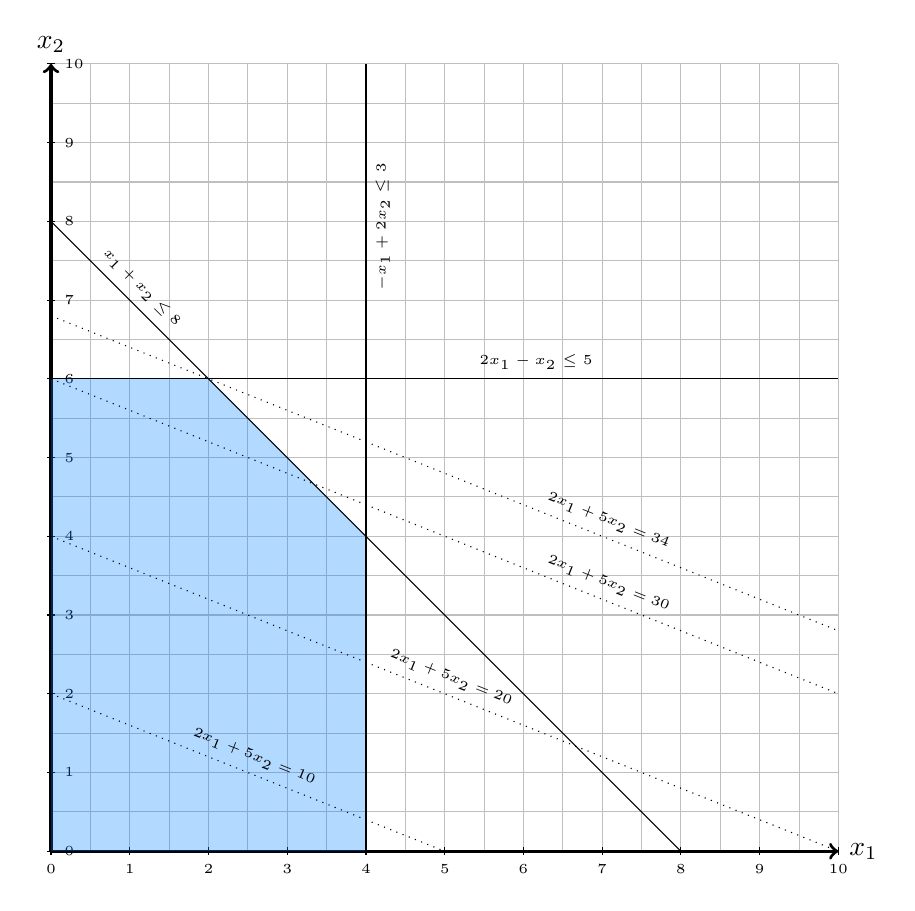
\begin{tikzpicture}

    \draw[gray!50, thin, step=0.5] (0,0) grid (10,10);
    \draw[very thick,->] (0,0) -- (10,0) node[right] {$x_1$};
    \draw[very thick,->] (0,0) -- (0,10) node[above] {$x_2$};

    \foreach \x in {0,...,10} \draw (\x,0.05) -- (\x,-0.05) node[below] {\tiny\x};
    \foreach \y in {0,...,10} \draw (-0.05,\y) -- (0.05,\y) node[right] {\tiny\y};

    \fill[blue!50!cyan,opacity=0.3] (0,0) -- (0,6) -- (2,6) -- (4, 4) -- (4, 0) -- cycle;

    \draw (0, 8) -- node[above,sloped] {\tiny$x_1+x_2\leq8$} (2, 6) -- (8,0);
    \draw (0, 6) -- (4, 6) -- node[above left,sloped] {\tiny$2x_1-x_2\leq5$} (10, 6);
    \draw (4, 0) -- (4, 4) -- node[below right,sloped] {\tiny$-x_1+2x_2\leq3$} (4,10);
    \draw[dotted] (0, 2) -- node[above, sloped] {\tiny$2x_1 + 5x_2 = 10$} (5, 0);
    \draw[dotted] (0, 4) -- node[above, sloped] {\tiny$2x_1 + 5x_2 = 20$} (10, 0);
    \draw[dotted] (0, 6) -- (4, 4.4) -- node[above, sloped] {\tiny$2x_1 + 5x_2 = 30$} (10, 2);
    \draw[dotted] (0, 6.8) -- (4, 5.2) -- node[above, sloped] {\tiny$2x_1 + 5x_2 = 34$} (10, 2.8);


\end{tikzpicture}

We can see from the dotted lines I've drawn in for different values of $c$ in\\ $2x_1 + 5x_2 = c$ 
that the maximum $c$ we will have is the top dotted line when\\ $c = 34, x_1 = 2, x_2 = 6$.

\end{problem}


\small
\bibliographystyle{amsalpha}
\bibliography{ref}


\end{document}





